\subsection{Impact of Datamix}
\label{sec:datamix_ablations}

Beyond our primary goal, which is to maximize support for low-resource languages while minimizing regressions in higher-resource ones, we also sought to build robustness against the wide range of noise conditions and speaker variability found in real-world audio. To meet these dual objectives, we designed a series of ablations and upsampling experiments tailored to the challenges of our \allasr{} dataset, which is both highly heterogeneous in audio quality and heavily imbalanced in language coverage.

\subsubsection{Upsampling Low-Resource Languages}

We upsampled at both the corpus- (datasource) and language-levels according to the following hyperparameters: \(\beta_c\)  and \(\beta_l\). \(\beta_c\) determines the relative weight assigned to a particular corpus, and \(\beta_l\) determines the relative weight for a particular language within a corpus. More precisely, for each corpus, we sampled language $L$ according to $p_l \sim \left( \frac{n_l}{N} \right)^{\beta_l}$, where $l = 1,...,L$ is the language, $n_l$ is amount of labeled ASR data for each language within the corpus, and $N$ is total volume of data in the dataset. Sampling across corpora was determined by treating each corpus as a language in the above equation, and using parameter $\beta_c$. This approach is consistent with previous work \citep{pratap2024scaling}. Lower beta values result in higher levels of upsampling of smaller data sources, with 0.0 causing uniform sampling across languages (irrespective of the amount of training data available for each language), and 1.0 representing a baseline where we simply concatenate all data without performing any upsampling.

To determine the optimal upsampling hyperparameters, we performed a sweep across different combinations of $\beta_c$ and $\beta_l$. For hyperparameter selection, we trained a 1B CTC model for 200K steps, and then compared results on all three evaluation protocols described in \Cref{section:eval}: resource-based (\Cref{tab:upsampling_cer_results_resource_bucket}), language-family (\Cref{tab:upsampling_cer_results_lang_family}), and corpus-based (\Cref{tab:upsampling_cer_results_corpus}).

Looking at \Cref{tab:upsampling_cer_results_resource_bucket}, we can see that as we increase language-level upsampling (ie, decrease $\beta_l$ at a given $\beta_c$), CERs decrease for low-resource languages. The baseline (1.0, 1.0) setting, which corresponds to no upsampling, performs by far the worst on low-resource languages. According to results on the resource-based protocol, the best setting is (0.0, 0.0), which is maximal (uniform) upsampling at both the corpus- and language-levels. This setting also gives the highest performance according to the language-grouping evaluation protocol, producing the lowest CERs within each grouping (see \Cref{tab:upsampling_cer_results_lang_family}). 

\Cref{tab:upsampling_cer_results_corpus} shows results on the corpus evaluation protocol. Here, the (0.5, 0.25) setting achieves best results in the corpus evaluation protocol. We can also see here that the (0.0, 0.0) setting obtained lowest CERs on MMS-lab corpus—which comprises over 1000+ languages. This helps explain why it performed so well on the language-based evaluation protocols: they are largely determined by the broad language coverage of MMS-lab. However, this increased MMS-lab performance came at the expense of other datasets such as Babel and CV22, which are known to contain noisier audio data and more diverse speaking conditions. As described subsequently in \Cref{sec:corpus_holdout_ablations}, over-indexing on the narrow audio domain of MMS-lab can have adverse effects on model robustness. Consequently, we chose the (0.5, 0.25) setting when training our final OmniASR models, as this performs well across all corpora and still achieves good results on the language-based protocols.

\begin{table}[htbp]
  \centering
  \begin{tabular}{l r r r r r r | r}
    \toprule
    Condition & Babel & MMS-lab & CV22 & FLEURS\_102 & MLS & OmniASR & Avg \\
    \midrule
    cbeta\_0.0\_lbeta\_0.0   & 27.55 & 4.47 & 17.73 & 9.64 & 3.86 & 24.08 & 14.55 \\
    cbeta\_0.25\_lbeta\_0.5  & 25.05 & 7.07 & 16.74 & 9.24 & 3.25 & 25.75 & 14.52 \\
    cbeta\_0.5\_lbeta\_0.5   & 25.71 & 6.32 & 17.14 & 9.63 & 3.26 & 26.23 & 14.71 \\
    cbeta\_0.75\_lbeta\_0.5  & 27.01 & 5.82 & 17.10 & 10.46 & 3.32 & 27.54 & 15.21 \\
    cbeta\_0.5\_lbeta\_0.25  & 25.41 & 6.05 & 16.42 & 9.42 & 3.32 & 26.08 & 14.45 \\
    cbeta\_0.5\_lbeta\_0.75  & 25.85 & 6.55 & 17.94 & 9.61 & 3.20 & 26.35 & 14.92  \\
    cbeta\_1.0\_lbeta\_1.0   & 28.72 & 6.09 & 21.30 & 11.15 & 3.20 & 29.33 & 16.63 \\
    \bottomrule
  \end{tabular}
  \caption{Performance (CER) across dev splits for each corpus in AllASR dataset for different $beta$ values. The rightmost column (avg) is separated for clarity.}
  \label{tab:upsampling_cer_results_corpus}
\end{table}


\begin{table}[htbp]
  \centering
  \begin{adjustbox}{max width=\textwidth}
  \begin{tabular}{l r r r r r r r}
    \toprule
    \multicolumn{8}{c}{\textbf{CERs for (cbeta, lbeta) upsampling}} \\
    \midrule
    \makecell{Language\\Groupings} & (0.0, 0.0) & (0.25, 0.5) & (0.5, 0.25) & (0.5, 0.5) & (0.5, 0.75) & (0.75, 0.5) & (1.0, 1.0) \\
    \midrule
    Afroasia   & 16.35 $\pm$ 3.11 & 18.70 $\pm$ 3.20 & 18.06 $\pm$ 3.18 & 18.45 $\pm$ 3.40 & 18.86 $\pm$ 3.94 & 17.96 $\pm$ 3.20 & 19.37 $\pm$ 4.12 \\
    Amazbasi   & 3.12 $\pm$ 0.41  & 5.04 $\pm$ 0.58  & 4.34 $\pm$ 0.52  & 4.39 $\pm$ 0.52  & 4.48 $\pm$ 0.55  & 4.13 $\pm$ 0.51  & 4.12 $\pm$ 0.57  \\
    Amerande   & 3.40 $\pm$ 0.72  & 4.95 $\pm$ 0.85  & 4.45 $\pm$ 0.85  & 4.55 $\pm$ 0.87  & 4.63 $\pm$ 0.88  & 4.48 $\pm$ 0.96  & 4.65 $\pm$ 1.13  \\
    Atlacong   & 12.43 $\pm$ 1.19 & 15.47 $\pm$ 1.15 & 14.70 $\pm$ 1.19 & 14.90 $\pm$ 1.19 & 15.05 $\pm$ 1.19 & 14.95 $\pm$ 1.25 & 15.62 $\pm$ 1.34 \\
    Austasia   & 11.80 $\pm$ 6.55 & 14.41 $\pm$ 6.32 & 12.88 $\pm$ 7.14 & 13.52 $\pm$ 7.14 & 13.98 $\pm$ 7.37 & 13.43 $\pm$ 7.29 & 14.19 $\pm$ 6.90 \\
    Austrone   & 6.63 $\pm$ 1.10  & 8.07 $\pm$ 1.11  & 7.76 $\pm$ 1.14  & 7.88 $\pm$ 1.14  & 7.99 $\pm$ 1.15  & 7.99 $\pm$ 1.20  & 8.35 $\pm$ 1.25  \\
    Caucasus   & 11.89 $\pm$ 4.39 & 11.95 $\pm$ 3.46 & 13.62 $\pm$ 5.10 & 12.58 $\pm$ 4.33 & 13.76 $\pm$ 5.24 & 13.13 $\pm$ 5.39 & 14.43 $\pm$ 5.16 \\
    Dravidia   & 13.16 $\pm$ 8.77 & 14.26 $\pm$ 7.57 & 13.73 $\pm$ 7.89 & 14.02 $\pm$ 7.73 & 14.02 $\pm$ 7.15 & 13.99 $\pm$ 7.80 & 14.08 $\pm$ 6.70 \\
    Indoeuro   & 13.15 $\pm$ 1.95 & 14.47 $\pm$ 1.99 & 14.35 $\pm$ 2.00 & 14.74 $\pm$ 2.02 & 15.15 $\pm$ 2.15 & 15.15 $\pm$ 2.09 & 17.25 $\pm$ 2.28 \\
    Mesoamer   & 10.53 $\pm$ 1.93 & 13.05 $\pm$ 1.88 & 12.36 $\pm$ 1.93 & 12.55 $\pm$ 1.92 & 12.67 $\pm$ 1.91 & 12.59 $\pm$ 1.99 & 13.21 $\pm$ 2.09 \\
    Newguine   & 7.27 $\pm$ 2.31  & 9.24 $\pm$ 2.39  & 8.68 $\pm$ 2.44  & 8.83 $\pm$ 2.44  & 8.97 $\pm$ 2.45  & 8.76 $\pm$ 2.55  & 9.07 $\pm$ 2.65  \\
    Nilosaha   & 7.23 $\pm$ 1.81  & 10.36 $\pm$ 1.76 & 9.25 $\pm$ 1.85  & 9.46 $\pm$ 1.86  & 9.69 $\pm$ 1.89  & 9.25 $\pm$ 2.01  & 9.51 $\pm$ 2.17  \\
    Norameri   & 8.22 $\pm$ 3.88  & 11.32 $\pm$ 3.77 & 10.08 $\pm$ 4.03 & 11.16 $\pm$ 4.40 & 12.11 $\pm$ 6.07 & 10.55 $\pm$ 4.24 & 13.40 $\pm$ 7.81 \\
    Sinotibe   & 13.72 $\pm$ 4.91 & 15.85 $\pm$ 4.93 & 14.88 $\pm$ 4.97 & 15.22 $\pm$ 5.03 & 15.85 $\pm$ 5.30 & 15.50 $\pm$ 5.34 & 16.97 $\pm$ 5.90 \\
    Misc       & 23.05 $\pm$ 2.46 & 24.54 $\pm$ 2.53 & 24.56 $\pm$ 2.54 & 24.82 $\pm$ 2.52 & 25.13 $\pm$ 2.50 & 25.68 $\pm$ 2.55 & 27.47 $\pm$ 2.57 \\
    \midrule
    \textbf{Average} & 10.80 $\pm$ 3.03 & 12.78 $\pm$ 2.90 & 12.25 $\pm$ 3.12 & 12.47 $\pm$ 3.10 & 12.82 $\pm$ 3.32 & 12.50 $\pm$ 3.22 & 13.44 $\pm$ 3.51 \\
    \bottomrule
  \end{tabular}
  \end{adjustbox}
  \caption{Performance (CER) across language groupings for different upsampling conditions. CER is averaged across all languages within each language family; error bars indicate 95\% Confidence Intervals.}
  \label{tab:upsampling_cer_results_lang_family}
\end{table}

\begin{table}[htbp]
  \centering
  \begin{tabular}{l r r r | r}
    \toprule
    Condition & High & Med & Low & \textbf{Avg} \\
    \midrule
    cbeta\_0.0\_lbeta\_0.0   & 6.28 & 6.12 & 21.14 & 11.18 \\
    cbeta\_0.25\_lbeta\_0.5  & 6.80 & 8.70 & 23.23 & 12.91 \\
    cbeta\_0.5\_lbeta\_0.5   & 6.54 & 8.08 & 23.42 & 12.5 \\
    cbeta\_0.75\_lbeta\_0.5  & 6.60 & 7.63 & 24.38 & 12.68 \\
    cbeta\_0.5\_lbeta\_0.25  & 6.54 & 7.86 & 23.09 & 12.89 \\
    cbeta\_0.5\_lbeta\_0.75  & 6.50	& 8.37 & 23.79 & 12.87 \\
    cbeta\_1.0\_lbeta\_1.0   & 6.75 & 8.09 & 26.40 & 13.75 \\
    \bottomrule
  \end{tabular}
  \caption{Performance (CER) across resource buckets and conditions for different $beta$ values. The rightmost column (Avg) is separated for clarity.}
  \label{tab:upsampling_cer_results_resource_bucket}
\end{table} 

\subsubsection{Generalizing to Unseen Audio Distributions}
\label{sec:corpus_holdout_ablations}

In addition to optimizing for low-resource languages, we also wanted to ensure our model was robust to various audio conditions. As such, we ran an ablation where we trained models on the \allasr{} dataset, holding out one corpus at a time. Here $AllASR$ refers to: MMS-lab, \vendorcorpus, OMSF, FLEURS-102, Babel, MLS, and CV22\footnote{Note this is a subset of \allasr{} used to train our final models. Refer to Table~\ref{tab:all_asr_dataset} for a list of all data sources}. For example, $AllASR\_x\_mls$ refers to a model trained on all of the above except MLS. We evaluates these $AllASR\_x$ holdout models on development splits from the held-out data sources, and compares them to a baseline model trained on the complete $AllASR$ dataset, thus measuring their ability to generalize to unseen audio distributions. 

Further, we contrasted these hold-out model conditions with a model trained on just MMS-lab. This latter model was still exposed to all languages in the hold-out sources, but it was not exposed audio from any other data sources. Comparing the $AllASR\_x$ holdout models against MMS-lab model allows us to assess the degree to which our model becomes better at generalizing to new audio distributions as we expand the training set to include more sources. In all conditions, we trained 1B CTC models for 100K steps at 32 GPUs.

\begin{table}
    \centering
    \begin{tabular}{llrrr}
    \toprule
         Training Data&  Holdout Data source&  Holdout CER&  Baseline CER& Baseline CERR\\
    \midrule
         AllASR\_x\_mls&  mls&  4.3&  3.27& -31\%\\
         AllASR\_x\_fleurs&  fleurs&  20.95&  11.95& -75\%\\
         AllASR\_x\_cv22&  cv22&  33.46&  19.57& -71\%\\
         MMS-lab&  mls&  6.34&  3.27& -94\%\\
         MMS-lab&  fleurs&  35.72&  11.95& -199\% \\
 MMS-lab& cv22& 43.35& 19.57&-1.22\\
    \bottomrule
    \end{tabular}
    \caption{Corpus holdout ablation results. Rows 1-3 contain performance for models  trained on our AllASR dataset, with a single source held-out from training. CERs for heldout corpora are shown in third column, and can be compared to CER obtained by a baseline model trained on all data (including the holdout corpus, fourth column). Rows 4-6 show holdout performance of a model trained on just MMS-lab, which covered all languages in the holdout corpora but had less audio diversity. Column 5 shows relative Character Error Rate reduction (CERR) of the holdout condition relative to the baseline: $(CER_{baseline} - CER_{treatment})/CER_{baseline}$. These values are all negative, indicating regressions for the holdout models compared to the baseline, which has seen all the data.}
    \label{tab:corpus_holdout_ablation_results}
\end{table}

Results are displayed in \Cref{tab:corpus_holdout_ablation_results}. Rows 1-3 show CERs obtained by $AllASR\_x$ models on their respective holdout corpora (column 3). These numbers can be compared against Baseline CERs obtained by the $AllASR$ model (column 4). Baseline CERR (column 5) makes this delta explicit: more negative values indicate larger regressions compared to baseline. As expected, performance regresses for all held-out data sources compared to the baseline.  The regression is more pronounced on FLEURS and CV22 than on MLS, suggesting that those two sources comprise more distinct audio distributions compared to the other sources within AllASR. That said, models still perform reasonably well on the holdout corpora (especially on MLS), indicating an ability to generalize to unseen audio distributions.

Crucially, Baseline CERR is substantially better in the $AllASR\_x$ models compared to the MMS-lab condition. This is true across all three holdout sources and indicates that our $AllASR$ recipe improves our model's ability to generalize to unseen audio distributions, as compared to training on a single data source with the same language coverage.

\subsubsection{Model Robustness to Background Noise}
\label{sec:noise_robustness}

Building on the previous section, we further examine model robustness by measuring ASR performance as a function of background noise and/or clarity of the speech signals. To do this, we ran audio samples in our development sets through the Torchaudio Squim models, which emit estimations of speech audio quality \citep{kumar2023squim}. \Cref{fig:cer_vs_sisdr} shows CER as a function of SI-SDR, which is a model estimate of the level of background noise relative to the speech signal. Model performance on different language groups is shown in different colors according to the resource-level (number of training hours) associated with each language. The analysis was performed on our 7B CTC model (solid line) as well as our 7B LLM-ASR model (dashed line).

\begin{figure}
    \centering
    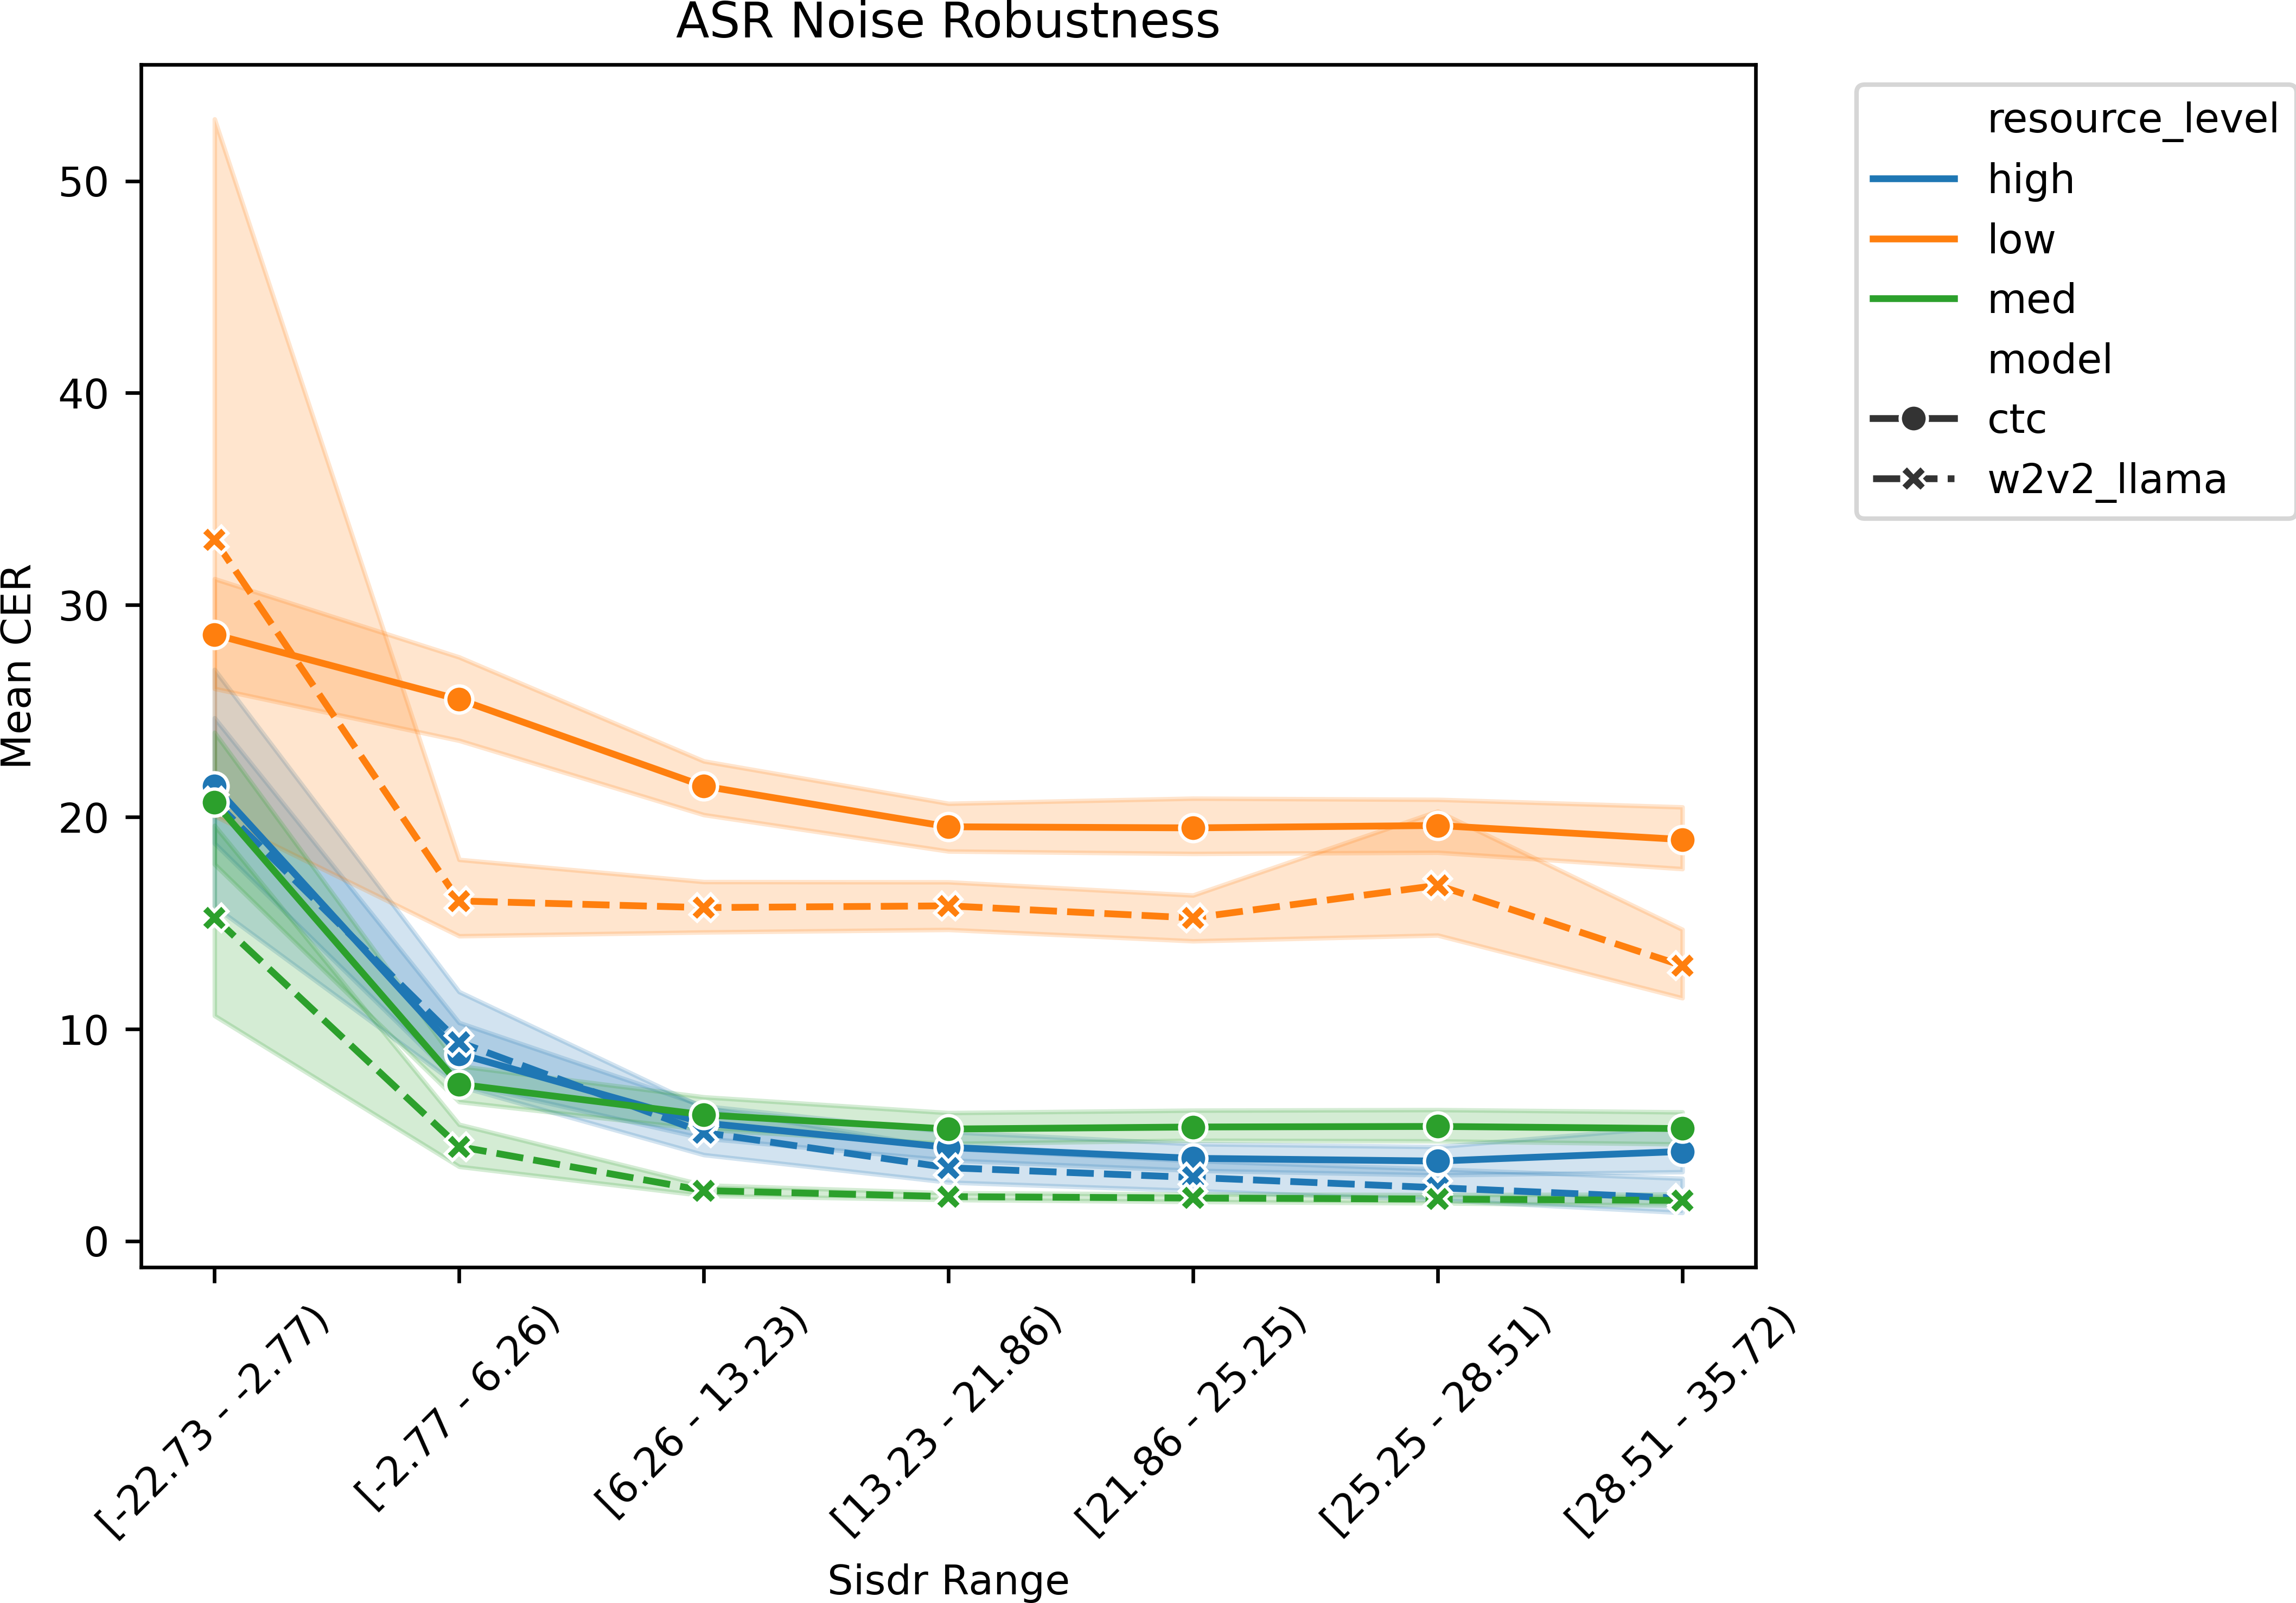
\includegraphics[width=0.75\linewidth]{assets/cer_vs_Sisdr_ctc_llama_custom_bins_unfiltered_tight.png}
    \caption{ASR noise robustness across All\_ASR dev sets. Utterances were binned into SI-SDR ranges that showcase the outliers with low SI-SDR values, up through the rest of the distribution. Mean CER values, averaged across languages (y-axis), are plotted against SI-SDR range (x-axis) of the associated audio. Error ribbons indicate 95\% CI. Results are further grouped by resource-level of the included language, as indicated by color: low- (orange; <10 hrs), medium- (blue; 10<=hours<50 hours), and high-resource (green; >50 hours). Results presented are for the 7B CTC model (solid line) and w2v2\_LLM (dashed line). Error ribbons indicate 95\% Confidence Intervals.}
    \label{fig:cer_vs_sisdr}
\end{figure}

Results are presented in \Cref{fig:cer_vs_sisdr}. Each utterance was binned into SI-SDR ranges, which were not evenly spaced but instead selected to showcase the extreme outliers in the distribution of our \allasr{} dataset (i.e., audios with large amounts of background noise). The ranges correspond to the following SI-SDR percentiles: [0-1, 1-5, 5-20, 20-40, 40-60, 60-80, 80-95, 95-100].  To remove any confounds with LID, we only include languages with utterances in each of the displayed SI-SDR bins. Within each SI-SDR bin, we obtain Mean CER (averaged across languages; y-axis) and plot this against SI-SDR bin-range (x-axis). Error ribbons indicate 95\% Confidence Intervals. CTC performance is indicated by dots/solid line, while LLM-ASR is indicated by x/dashed line. Languages with different levels of training data are grouped by color: low-resource (<10 hours), medium-resource (between 10-50 hours), and high-resource (>50 hours). 

As expected, CER is higher for utterances with low SI-SDR values (high background noise) compared to utterances with higher SI-SDR (cleaner audio). CER is highest and most variable at the extreme low-end (lowest 1\% of SI-SDR).  However, CER quickly drops and flattens out after this. For instance, even for the noisiest 1\%-5\% of utterances, LLM-ASR model obtains CERs $\leq 10$ across all language groups, and the CTC model obtains CERS $<15$ for medium- and high-resource languages. In the remaining SI-SDR bins, CER is quite flat within each language group. It is important to recall that the x-axis in \Cref{fig:cer_vs_sisdr} is not a linear scale throughout: the first two bin-ranges represent outlier utterances with extreme levels of background noise (i.e., top 1\% and top 5\%, respectively). Overall, these results indicate good model robustness to moderate levels of background noise (i.e., lowest 5\% percentiles), and that our models do not exhibit any bias in background noise sensitivity as a function of language resource-level.

\subsubsection{\vendoromsf Holdout Ablation}
\label{sec:omni_asr_corpus_holdout}

To measure the value of the \vendoromsf data (i.e., all the new data collected in this project: \vendorcorpus plus OMSF), we ran a simple ablation in which we compared a \allasr{} model against an \allasr{}\_x\_\vendoromsf model.  In the latter, we held out \vendoromsf data from training and then evaluated the model on the hold-out \vendoromsf dev sets. In both conditions, we trained 7B LLM-ASR models for 150K steps across 64 GPUs.

To be clear, \vendoromsf introduces mostly new languages to the mix, so in these cases, the \allasr{}\_x\_\vendoromsf is being evaluated on languages it was not exposed to during training. In these cases, we expect the \allasr{} model to outperform the holdout model. Nevertheless, we include the ablation results to validate the training signal in \vendoromsf; this allows us to ensure that our claims of supporting newly introduced languages are well founded.

Additionally, there are 13 overlapping languages in \vendoromsf that are also contained in other corpora within \allasr{}. For these languages, we would like to see if the additional \vendoromsf training data provides a valuable signal above and beyond what was already present in our training data, especially with regard to speaker diversity and more naturalistic audio conditions. We separately report ablation results for new and overlapping languages in \Cref{tab:omni_holdout_ablation}.

\begin{table}
    \centering
    \begin{tabular}{rll}
        \toprule
         Data Condition & \makecell{CER\\(new languages)} & \makecell{CER\\(overlap langs)} \\
         \midrule
         $AllASR\_x\_OMNI$ & 47.03 & 39.46 \\
         $AllASR\_OMNI$ & 22.62 & 11.50 \\
    \bottomrule
    \end{tabular}
    \caption{\vendoromsf holdout ablation results. Mean CERs on the \vendoromsf dev sets, averaged across languages are shown for the holdout and full-data conditions. Results reported separately for new languages introduced by \vendoromsf versus languages that were already present in other corpora within \allasr{}.}
    \label{tab:omni_holdout_ablation}
\end{table}

Results in \Cref{tab:omni_holdout_ablation} highlight the value of the \vendoromsf data collected in this project, both by extending coverage to new languages and by substantially improving performance on already-supported ones. For new languages, our AllASR\_OMNI model achieves a mean CER of 22.62, less than half the 47.03 obtained by the holdout model. Although 22.62 remains relatively high compared to CERs obtained on other corpora, it nevertheless represents a major reduction from the holdout model’s zero-shot performance, despite that model being highly multilingual. For overlapping languages, the impact of \vendoromsf data is even more striking: CERs drop from 39.46 with the holdout model to 11.50 with AllASR\_OMNI.

This latter result underscores the fact that data from \vendoromsf is quite challenging for ASR compared to many pre-existing multilingual datasets, which mostly consist of clean, studio-quality recordings of speaker-reading. \vendoromsf was intentionally curated to represent naturalistic (i.e., often noisy) audio conditions, diverse speaker identities, and spontaneous, expressive speech. The benefits of such data are demonstrated here: without including them in the datamix, an equally multilingual model (i.e., our holdout) struggles in these more difficult, but more naturalistic audio/speaker conditions. In sum, by including \vendoromsf, we introduce new language coverage and also substantially improve model robustness, which ultimately situates our models for use in the wild.

\subsubsection{Fine-tuning for Individual Low-Resource Languages}
\label{sec:language_specific_ablations}

In this study, we fine-tuned bespoke CTC models on individual low-resource languages. There are two motivations here. First, from a theoretical standpoint, we are interested in establishing the best performance achievable for languages with fewer than 10 hours of data, and in quantifying the performance gap relative to our \OmniASR{} models trained across 1,600+ languages. Second, we present our learnings to the community to provide recommended settings for users interested in adapting and optimizing our open-source models for their own bespoke purposes, especially in lower compute settings. This study was performed with 11 low-resource languages, with between 5-10 hours of training data and at least 1 hour of validation splits. See \Cref{tab:low_res_lang_list} for the complete list.

\begin{table}
    \centering
    \begin{tabular}{llrr}
    \toprule
         LID & Script &  \# train hours& Best CER\\
    \midrule
         ast&Latn& 8.1 & 3.31 \\
         ckb&Arab& 9.1 & 4.47 \\
         ltz&Latn& 8.5 & 7.42 \\
         hsb&Latn& 9.1 & 2.17 \\
         afo&Latn& 7.6 & 29.7 \\
         ahl&Latn& 7.2 & 16.47 \\
         div&Thaa& 7.6 & 5.16 \\
         fuv&Latn& 6.5 & 15.1 \\
         qxp&Latn& 9.9 & 1.61 \\
         ajg&Latn& 9.5 & 8.05 \\
         vro&Latn& 9.5 & 5.7 \\
    \bottomrule
    \end{tabular}
    \caption{Low-resource languages used in language-specific study.}
    \label{tab:low_res_lang_list}
\end{table}

We fine-tuned language-specific CTC models for each of these 11 languages, across the 300M, 1B, and 3B scales. In one condition, we seeded from a pretrained w2v2 checkpoint, and in another, we seeded from an OmniASR CTC checkpoint, which was pretrained on all 1600+ languages. For the w2v2-seed condition, we trained with a learning rate of 1e-05 for 30K steps, though we observed that models typically converge within 10K steps. For the CTC-seed condition, we also use an lr of 1e-05 and trained for 5K steps. CTC fine-tuning takes \~1 hour of walltime on 32 GPUs for the 300M scale. These hyperparameters were selected based on empirical sweeps for a couple of exemplar languages, but of course, in practice, the optimal training hyperparameters will be a function of the specific language and data used in finetuning. For example, we observed that certain languages converged long before the \# training steps listed here.

We then compare the performance (CER) of these language-specific models against our \OmniASR CTC models at each scale. These \OmniASR models were trained on all 1600+ languages, without any sort of language-specific optimization. Results can be found in \Cref{tab:cer_per_low_res_language}. Language-specific models substantially outperform the \OmniASR baselines, achieving CERs of less than 5 in many of these low-resource languages—even at the smaller 300M and 1B scales. Additionally, CTC-seeded models consistently outperformed w2v2-seeded models at the 300M and 1B scales, even though they were fine-tuned for a fraction of the training steps (5K instead of 30K). Consequently, we advise practitioners wishing to optimize our 300M and 1B models for ASR in particular low-resource languages to seed with CTC checkpoints. However, at the 3B scale the w2v2-seeded checkpoints trained for 30K steps generally outperformed the ctc-seeded checkpoints trained for 5K steps.

\Cref{tab:cer_per_low_res_language} also shows CERs obtained by our 7B OmniASR LLM model in the rightmost column. In most cases, the OmniASR 7B-LLM was quite competitive with the language-specific models, indicating an extremely high performance on these low-resource languages despite the fact that it was trained on all 1600+ languages and without any language-specific optimization. On the other hand, even though the language-specific models are significantly smaller than the 7B-LLM model and lack the LLM architectural component, they still obtained lower CERs for most languages, even at the smallest 300M scale. This demonstrates a unique strength of our open-source \OmniASR models: they contain rich omnilingual knowledge, and can be quickly adapted and fine-tuned to excel in particular low-resource settings with minimal compute. Once fine-tuned, the lightweight CTC models can be run in small compute environments during inference, which can be desirable in numerous applications.

\begin{table}[htbp]
  \centering
  \begin{tabular}{ll
                  >{\raggedleft\arraybackslash}p{1.7cm}
                  >{\raggedleft\arraybackslash}p{1.7cm}
                  r | r}
    \toprule
    Language & Scale & \multicolumn{2}{c}{Single-Lang} & OmniCTC & \multicolumn{1}{c}{OmniLLM (7B)} \\
    \cmidrule(lr){3-4}
    & & CTC Seed & W2V2 Seed & & \\
    \midrule
    afo\_Latn & 300m & 32.54 & 32.32 & 33.54 & 38.91 \\
              & 1b   & 31.58 & 29.71 & 33.17 &       \\
              & 3b   & 30.89 & 29.11 & 32.18 &       \\
    \cmidrule(lr){1-6}
    ahl\_Latn & 300m & 18.78 & 20.52 & 44.28 & 24.33 \\
              & 1b   & 17.66 & 16.47 & 36.76 &       \\
              & 3b   & 17.87 & 15.27 & 34.61 &       \\
    \cmidrule(lr){1-6}
    ajg\_Latn & 300m & 8.05  & 8.63  & 21.97 & 7.54  \\
              & 1b   & 8.82  & 8.11  & 19.14 &       \\
              & 3b   & 9.02  & 7.92  & 15.63 &       \\
    \cmidrule(lr){1-6}
    ast\_Latn & 300m & 4.95  & 8.02  & 10.87 & 5.105 \\
              & 1b   & 3.55  & 4.83  & 7.88  &       \\
              & 3b   & 3.91  & 3.31  & 6.44  &       \\
    \cmidrule(lr){1-6}
    ckb\_Arab & 300m & 5.82  & 8.01  & 15.29 & 4.73  \\
              & 1b   & 5.05  & 5.91  & 12.28 &       \\
              & 3b   & 5.20  & 4.17  & 9.94  &       \\
    \cmidrule(lr){1-6}
    div\_Thaa & 300m & 5.54  & 8.36  & 19.21 & 5.58  \\
              & 1b   & 5.16  & 5.66  & 17.21 &       \\
              & 3b   & 5.45  & 4.57  & 13.04 &       \\
    \cmidrule(lr){1-6}
    fuv\_Latn & 300m & 16.41 & 18.45 & 23.69 & 26.83 \\
              & 1b   & 15.59 & 15.10 & 20.47 &       \\
              & 3b   & 15.14 & 14.35 & 16.31 &       \\
    \cmidrule(lr){1-6}
    hsb\_Latn & 300m & 2.93  & 7.18  & 10.41 & 4.1   \\
              & 1b   & 2.57  & 2.17  & 7.07  &       \\
              & 3b   & 3.20  & 1.79  & 4.94  &       \\
    \cmidrule(lr){1-6}
    ltz\_Latn & 300m & 9.88  & 15.94 & 19.72 & 6.07  \\
              & 1b   & 7.42  & 10.72 & 12.44 &       \\
              & 3b   & 8.09  & 7.12  & 9.80  &       \\
    \cmidrule(lr){1-6}
    qxp\_Latn & 300m & 1.70  & 2.08  & 4.49  & 1.32  \\
              & 1b   & 1.61  & 1.68  & 2.94  &       \\
              & 3b   & 1.81  & 1.47  & 2.71  &       \\
    \cmidrule(lr){1-6}
    vro\_Latn & 300m & 7.18  & 9.39  & 16.74 & 4.02  \\
              & 1b   & 6.36  & 5.70  & 12.67 &       \\
              & 3b   & 6.76  & 5.12  & 10.16 &       \\
    \bottomrule
  \end{tabular}
  \caption{Model performance (CER) across low-resource languages and scales. Columns 3-4 show language-specific models. The rightmost column (OmniLLM (7B)) is separated for clarity.}
  \label{tab:cer_per_low_res_language}
\end{table}